%-------------------------------------------------------------------------------
\section{Evaluation}
%-------------------------------------------------------------------------------

We evaluate Gradient Analysis both by comparing it with taint as a method of dataflow analysis, and in direct applications for vulnerability detection. Specifically, we run experiments to answer the following questions:

\begin{itemize}
  \item Does gradient analysis add more overhead than taint analysis?
  \item Is gradient analysis more accurate than taint analysis in predicting dataflows?
  \item Does using gradient analysis to guide fuzzing lead to better coverage?
  \item Can gradient analysis detect recent CVEs that taint is typically used to detect?
  \item Is gradient analysis an effective tool for vulnerability discovery?
\end{itemize}

\subsection{Test Programs}

We perform tests on a set 5 widely used file parsing libraries and 7 total programs. We select these programs to cover most common file types that must be routinely parsed and rendered from untrusted sources, and therefore are common vectors for attacks.

\begin{table}
\centering
 \begin{tabular}{ll l l} 
 \toprule
  Library & Test Program & SLOC & File Format \\ 
 \midrule
 zlib-1.2.11    & \verb|minigzip -d| & \gabe{TODO}    & GZ/ZIP \\ 
 mupdf-1.14.0   & \verb|mutool show| & 123,562    & PDF \\  
 libxml2-2.9.7  & \verb|xmllint| & 73,920    & XML \\
 libjpeg-9c     & \verb|djpeg| & 8,857    & JPEG \\
 %harfbuzz-1.7.6 & \verb|minigzip -d| &  9,853   & TTL \\
                & \verb|readelf -a| & 21,647    &  \\  
 binutils-2.30  & \verb|objdump -xD| & 72,955  & ELF \\  
                & \verb|strip | &  56,330   &  \\  
 \bottomrule
 \end{tabular}
  \caption{Summary of parser programs used in evaluation. \gabe{TODO compile with gcov to get linecounts  }}
  \label{tab:programs}
\end{table}


\subsection{Taint Tracking Comparison}

Since proximal gradient analysis is a new form of dynamic dataflow analysis, we focus most of our evaluation on comparisons with dynamic taint tracking, which is the most widely used version of dynamic dataflow analysis. For our comparison, we use the implementation of taint tracking in LLVM's DataFlowSanitizer. Since our implementation of proximal gradient analysis is based on the DataFlowSanitizer architecture, we ensure that differences in performance on evaluation tasks are due to the differences between gradient and taint as dataflow methods, and not any differences in the underlying frameworks or architecures used in their implementation. 

We compare proximal gradient analysis with taint tracking in three areas: first, we evaluate the overhead introduced by the dataflow tracking instrumentation. Second, we estimate the accuracy of the dataflows predicted by gradient and taint by perturbing input bytes. Third, we compare the coverage achieved by a fuzzer using gradient and taint predictions as a guide. 


\subsubsection{Performance Overhead}

We first address the question of how much overhead the instrumentation for gradient analysis adds to a program. To measure overhead, we first execute each program 50 times to ensure cache locality, and then execute 5000 times while recording runtime. Since individual executions of the test programs usually complete in less than a kernel tick (1 millisecond), we measure walltime instead of cpu time for all 5000 executions and compute mean runtime from that. We measure overhead for each program on a small input file, where the inputs range in size from 3.7Kb for JPEG to 8.5Kb for ELF. \gabe{can rerun with files of more similar size if needed.} The evaluation was performed on an Ubuntu 16.04 server with an Intel Xeon E5-2623 v4 2.60GHz CPU.

Table \ref{tab:performance} shows the results of the overhead comparison. \gabe{I feel like there are several things we need to sort out before discussing these results. In particular, some of the numbers are essentially identical for unlabeled vs labeled, and I'm not really sure why gradient is so much faster for libxml while slower for mupdf. Need to investigate which instructions are actually being processed to explain this intelligently. Also, may need to rerun with higher optimization than -O0 to see meaningful differences between labeled and unlabeled.}



\begin{table*}[t]
\begin{tabular}{@{}lllllllllll@{}}
\toprule
  & Base & \multicolumn{2}{c}{Unlabeled Taint} & \multicolumn{2}{c}{Unlabeled Gradient} & \multicolumn{2}{c}{Taint} & \multicolumn{2}{c}{Gradient} & Relative\\

  Program & Runtime & Runtime & Overhead & Runtime & Overhead & Runtime & Overhead & Runtime & Overhead & Overhead \\ 
\midrule
zlib & 0.00093 & 0.0015 & 0.56 & 0.0016 & 0.73 & 0.0015 & 0.57 & 0.0017 & 0.85 & 0.28 \\
jpeg & 0.00089 & 0.0014 & 0.59 & 0.0014 & 0.6 & 0.0015 & 0.63 & 0.0015 & 0.63 & -0.0017 \\
mupdf & 0.0031 & 0.0086 & 1.8 & 0.01 & 2.4 & 0.0086 & 1.8 & 0.01 & 2.4 & 0.59 \\
libxml & 0.0017 & 0.0072 & 3.2 & 0.0052 & 2.1 & 0.0072 & 3.2 & 0.0053 & 2.1 & -1.1 \\
readelf & 0.0012 & 0.0017 & 0.4 & 0.0017 & 0.41 & 0.0017 & 0.41 & 0.0018 & 0.46 & 0.046 \\
objdump & 0.0021 & 0.0021 & 0.017 & 0.0021 & 0.021 & 0.0021 & 0.016 & 0.0022 & 0.028 & 0.011 \\
strip & 0.0011 & 0.0022 & 0.95 & 0.0022 & 0.94 & 0.0022 & 0.96 & 0.0022 & 0.95 & -0.015\\ \bottomrule
\end{tabular}
 \label{tab:performance}
 \caption{Summary of performance. \gabe{Possibly add in ablation with label reuse optimization.}}
\end{table*}




\subsubsection{Dataflow Precision}

One of the main advantages gradient has over taint is that it naturally handles operations where numerical effects cause the input to have no effect on the output. These types of effects result in many situations where taint rules over approximate, marking large portions of the program as tainted when they are not and limiting the usefulness of taint as a tool for analysis. 

However, evaluating the extent to which overtainting occurs is difficult due to the exponential size of possible inputs. In theory, each possible input could be sampled to evaluate which input bytes can potentially effect a given internal program value and create a ground truth against which different dataflow methods could be evaluated. In practice complete evaluation is impossible so we sample a subset of possible inputs as follows: for each byte in the input that is predicted by taint, we generate sample inputs where the byte is set to 0, 255, and where each bit in the byte was toggled by 1 for a total of 10 samples per byte. We found that in practice this strategy usually resulted in a change to branch variables if it was possible to effect a change, since common patterns in branching were checking for 0, above or below a threshold, or if particular bits were set.

For our evaluation of precision we focus on branch constraints since these values most significantly effect the behavior of a program and are key to achieving good test coverage. Typically when dataflow is used in dynamic testing applications branch inputs are marked a sinks. \gabe{We could also mark a set of other functions if that makes sense.} For each branch input and each marked byte, we evaluate precision by recording its values over executions of all the input samples generated by modifying the byte. If any the modified inputs cause the branch value to change during execution, we consider that byte to have a valid dataflow to the branch input. 

We evaluate dataflow precision for taint and gradient on the parsing programs shown in table ~\ref{tab:programs} using a set of inputs generated by running afl on each program for an hour then running afl-cmin on the result. The results are shown in table (2) ~\ref{tab:precision_comp}. Gradient analysis is more precise than taint for all programs, although in some programs such as \tc{mutool} and \tc{xmllint} this improvement is relatively small. Overall, gradient is on average 32\% more precise than taint, as as much 42\% more precise for dataflow predictions on jpeg. We hypothesize that gradient gives a more significant improvement in accuracy when programs contain a large number of numerical operations, which often cause overtainting but are handled correctly by gradient. This effect can be seen in the large improvements for \tc{minigzip} and \tc{djpeg}, both of which use a large number of numerical operations to perform decompression on their inputs.

\gabe{TODO rerun this with recall recorded, calc f1, try to get higher coverage for readelf. Also would be nice to analyze what instructions are being instrumented here too and see how more sampling improves precision. Also add number of instrumented branches for each program, big numbers are impressive.}

\begin{table}
\centering
  \begin{tabular}{lrrr} 
 \toprule
    Test Program & Taint & Gradient & Relative \\ 
                 & Precision & Precision & Improvement \\ 
 \midrule
   minigzip (zlib-1.2.11)  & 0.593     & 0.917 & 0.324\\ 
   mutool (mupdf-1.14.0)   & 0.704     & 0.714 & 0.011\\
   xmllint (libxml2-2.9.7) & 0.957     & 0.988 & 0.032\\
   djpeg (libjpeg-9c)      & 0.519     & 0.942 & 0.423\\  
   readelf (binutils-2.30) & 0.074     & 0.075 & 0.001\\  
   objdump (binutils-2.30) & 0.352     & 0.516 & 0.163\\  
   strip   (binutils-2.30) & 0.344     & 0.585 & 0.241\\  
 \bottomrule
 \end{tabular}
 \caption{\label{tab:precision_comp}Summary of precision comparison results for taint and gradient Analysis.\abhi{need F1 score/recall}}
\end{table}



\subsubsection{Dataflow Guided Fuzzing}

Since dynamic dataflow analysis is often used as a tool to guide fuzzing, we next evaluate gradient analysis as a method for guided fuzzing. In order to perform a controlled comparison with taint tracking, we use the following procedure: first, the program under test is instrumented with dataflow method currently being tested, either gradient or taint, and modified to mark inputs when it processes a file. In addition, all of the programs branches are instrumented as sinks, so that dataflows to each branch from each input byte are recorded. The program is then executed on a single seed input, and the number branches each input byte has a dataflow to is recorded. The top 512 bytes are then selected based on the number of branches they effect, and targeted for fuzzing. 

To perform the fuzzing, we use a modified implementation of AFL that uses a strategy formulated for targeted important bytes. The fuzzer first targets each byte individually, and then doubles the number of bytes targeted in each subsequent search until it has targeted all selected bytes. When bytes are targeted individually all possible values are searched exhaustively, while when multiple bytes are targeted, a single direction for mutations is selected and each byte is randomly incremented or decremented until it reaches its maximum or minimum value. \gabe{Dongdong you'll need to double check all this is correct. Also, is this the search strategy from neuzz? If so we should cite it (or something else that helps justifying it.)}

Once the first seed has been fully searched, we perform the same dataflow procedure on all generated seeds to identify their most influential bytes and then fuzz each one in turn. We record the overall coverage on the program under test for both gradient and taint every 100 thousand mutations, up to 1 million mutations.

See figure ~\ref{fig:fuzz_comp} for results. \gabe{Discuss results here. Lots of discussion. Yup lots of things to discuss. As soon as we results. Our method is certainly much better, that's for certain. No doubt the results will show that.}

\begin{figure*}[t]
  \centering
  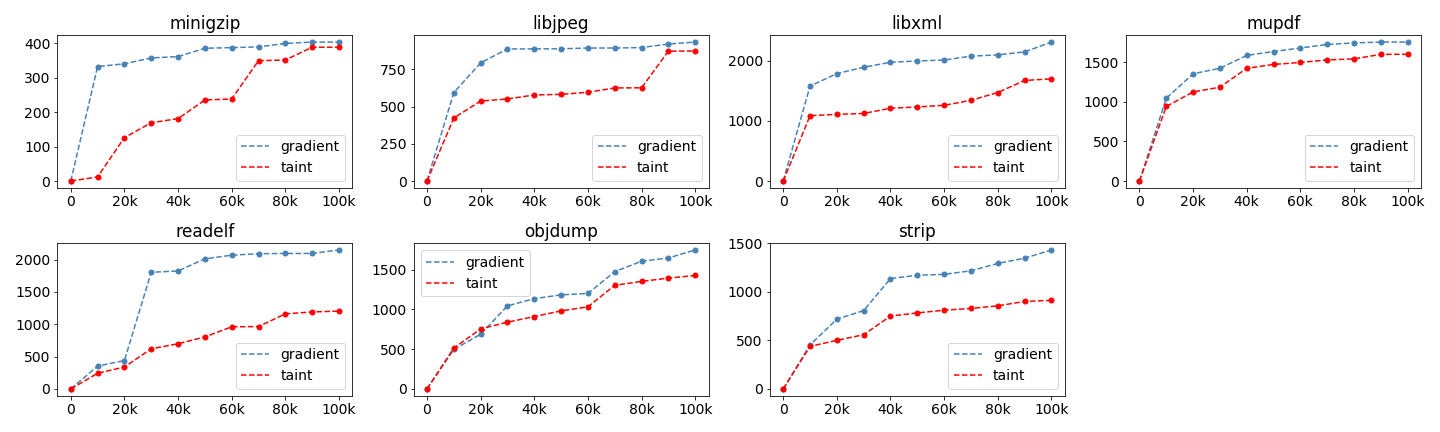
\includegraphics[width=\linewidth]{figs/fuzz_comp_plot}
  \vspace{-10pt}
   \caption{ \label{fig:fuzz_comp}Comparison of guided fuzzer coverage achieved by gradient and taint analysis over 1 million mutations from a single seed.}
  \vspace{-10pt}
\end{figure*}


\begin{table*}[t]
\centering
  \begin{tabular}{l r rr rr} 
 \toprule
    & & \multicolumn{2}{c}{Taint Guided} & \multicolumn{2}{c}{Gradient Guided} \\ 
    \cmidrule(r){3-4} \cmidrule(r){5-6}
    Test Program & Original Edges  & Final Edges & \# Executions &  Final Edges & \# Executions\\ 
 \midrule
   minigzip (zlib-1.2.11)  &      &  &  &  &   \\ 
   mutool (mupdf-1.14.0)   & 2114     & 3509 & 3667  & 3551 & 3667  \\
   xmllint (libxml2-2.9.7) & 3573      &   4085   & 2400   &   4288   &  2400      \\
   djpeg (libjpeg-9c)      & 1259     & 2067     &   285420    & 2160 & 285420 \\  
   readelf (binutils-2.30) & 1379      & 1609  & 2994 & 1795  & 2994  \\  
   objdump (binutils-2.30) & 2804     & 3167 &3352  & 3426 & 3352  \\  
   strip   (binutils-2.30) & 2603     & 3191 & 3155 & 3624 & 3155  \\  
 \bottomrule
 \end{tabular}
  \caption{\label{tab:fuzzer_comp}Summary of guided fuzzing coverage comparison results for Taint and Gradient Analysis. \gabe{Temporarily keeping this for reference but will replace with figure \ref{fig:fuzz_comp}}}
\end{table*}

\subsection{Bug Finding}

In addition to performing comparative evaluations of gradient with taint tracking, we also evaluate its utility as a tool for finding bugs in real world programs. We test gradient analysis in three applications: detecting attacks at runtime, guiding discovery of new vulnerabilities, and discovering information leaks.


\subsubsection{CVE-detection}

We first evaluate gradient analysis as tool for detecting attacks at runtime, which is the application dynamic taint analysis was originally designed for. To detect the attacks, we instrument the programs so that the gradients of parameters of instructions involved in the attack are recorded. As shown in table ~\ref{tab:cve_detection}, we test X known attacks against all 7 programs and demonstrate gradient analysis can detect all X attacks. This result shows that gradient can perform that same task as dynamic taint analysis as a baseline. \gabe{If we can generate an input that triggers a detectable error by gradient but makes dfsan run out of labels we can also talk about that. }

\begin{table}
\begin{tabular}{l l l}
\toprule
CVE ID & Vulnerability & Program \\
\midrule
CVE-2018-10372 & heap overflow & readelf  \\
CVE-2018-6759 & null pointer dereference & nm  \\
CVE-2018-19932 & integer overflow & strip  \\
\bottomrule
\end{tabular}
\caption{\abhi{TODO}}
  \label{tab:cve_detection}
\end{table}


\subsubsection{Bug Discovery}

After evaluating gradient analysis as a tool for detecting known attacks, we next evaluate the utility of gradient analysis in discovering new bugs in programs. To do so we add additional instrumentation to record gradients for instruction and function arguments that can potentially trigger program errors, such as memory allocations, copy instructions, indexing operations, and shift operators. We then execute the programs on a corpus of files generated by running AFL on each program for 24 hours, as well as a selection of files generated from other programs to further extend coverage. For each file, if any input bytes have a nonzero derivative with an instrumented function, we generate new inputs using the function gradient as a guide. For most functions we generate inputs setting the bytes with a gradient to either 0 or 255, although for instructions can potentially trigger a division by 0 we also search all possible values for each byte.

Table ~\ref{tab:bug_summary} summarizes our results. Overall we find X bugs across all 7 programs, including buffer overflows, memory allocations, integer overflows, and division by 0. \gabe{Discuss these results more when we a better bug count.}

\begin{table}
\centering
 \begin{tabular}{ll l l} 
 \toprule
  Library & Test Program & Arithmetic & Memory \\ 
 \midrule
 zlib-1.2.11    & \verb|minigzip -d| &     &  \\ 
 mupdf-1.14.0   & \verb|mutool show| &     &  \\  
 libxml2-2.9.7  & \verb|xmllint| &     &  \\
 libjpeg-9c     & \verb|djpeg| & 3    &  \\
 %harfbuzz-1.7.6 & \verb|minigzip -d| &  9,853   & TTL \\
                & \verb|readelf -a| &     &3  \\  
  binutils-2.30 & \verb|objdump -xD| & & 1 \\  
                & \verb|strip | &     & 6 \\  
 \bottomrule
 \end{tabular}
  \caption{Summary of bug types found by Gradient Analysis for parser programs.}
  \label{tab:bug_summary}
\end{table}



\subsubsection{Information Leak Discovery}

Finally, we evaluate gradient analysis as tool for discovering information leaks in programs. Side channel attacks that take advantage of information leaks in systems are a common method for bypassing traditional security measures. To evaluate gradient analyis as a method for assessing vulnerability to these types attacks, we... \gabe{I'm not quite sure yet, this will probably involve looking at gradients to branches or memory allocations from specific fields in the input.}

Table \ref{tab:information_leaks} summaries our results. We find X information leaks in total across Y programs, and use gradient analysis to identify how the leaks occur in the programs. 


\begin{table}
\begin{tabular}{l l l}
\toprule
Program & Leaked Data & Leak Vector \\
\midrule
mutool & content header type & runtime \\
minigzip & compression type & runtime \\
objdump & note header size & memory usage \\
\bottomrule
\end{tabular}
  \caption{\label{tab:information_leaks} Examples of information leaks identified with gradient analysis. \gabe{This is just a filler table.}}
\end{table}
